\documentclass[handout]{beamer}

\usepackage[english]{babel}
\usepackage[latin1]{inputenc}
\usepackage[T1]{fontenc}
\usepackage{graphicx}
\usepackage{geometry}
\usepackage{amsmath,amssymb}
\usepackage{epstopdf}
\usepackage{url}



%\usetheme{Marburg}
%\usetheme{Berkeley}
\usetheme{PaloAlto}
%\usetheme{Warsaw}


\AtBeginSection[]
{
  \begin{frame}
  \frametitle{Sommaire}
  \tableofcontents[currentsection, hideothersubsections, pausesubsections]
  \end{frame} 
}



\title{\textbf{Top-Down and Bottom-up Cues for Scene Text Recognition, \\
 A. Mishra, K. Alahari, C. V. Jawahar}}
\author{Vincent BODIN \& Thomas MOREAU}




\begin{document}

\renewcommand{\contentsname}{Sommaire}


\begin{frame}[allowframebreaks]
\titlepage
\end{frame}


\section*{Introduction}


\begin{frame}{Introduction}
\begin{figure}%
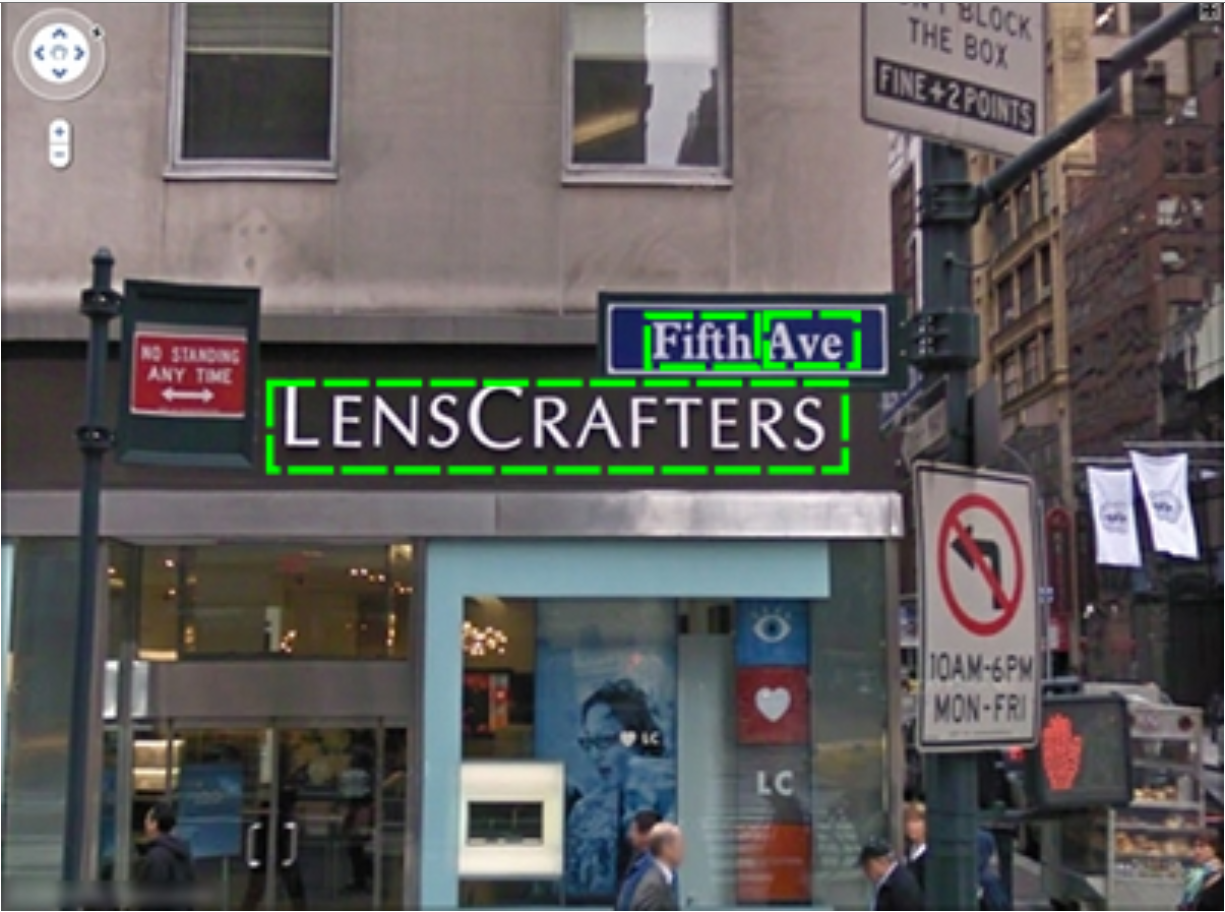
\includegraphics[width=9cm]{figures/intro.png}%
\caption{Task of the project (image from SVT)}%
\label{}%
\end{figure}
\end{frame}




\section{Learning preliminaries}

\subsection{Learning characters}

\begin{frame}{Learning characters}
We need to build classifiers to recognize characters in a natural picture:
\begin{enumerate}
	\item Character databases: ICDAR 2003 \cite{ICDARchar}, Chars74K \cite{Char74K};
	
	\item features: Histogram Of Gradient (HOG) \cite{Dal2005}\footnote{N. Dalal, B. Triggs, Histogram of oriented gradients for human detectection};
	
	\item build $K$ SVMs ($K = 62$) with RBF Kernel, Fig.(\ref{RBFKernel}):
	\begin{equation}
	\exp(-\gamma |x-x'|^2), \gamma > 0
	\label{eq:}
	\end{equation}
	method one-versus-all, we used a Python library scikit-learn \cite{scikit}: $K$ coefficients $\gamma$ and regularization $C$ optimized by cross-validation => test error without optimization $25\%$, with optimization $16\%$.
\end{enumerate}
\end{frame}


\begin{frame}
\begin{figure}%
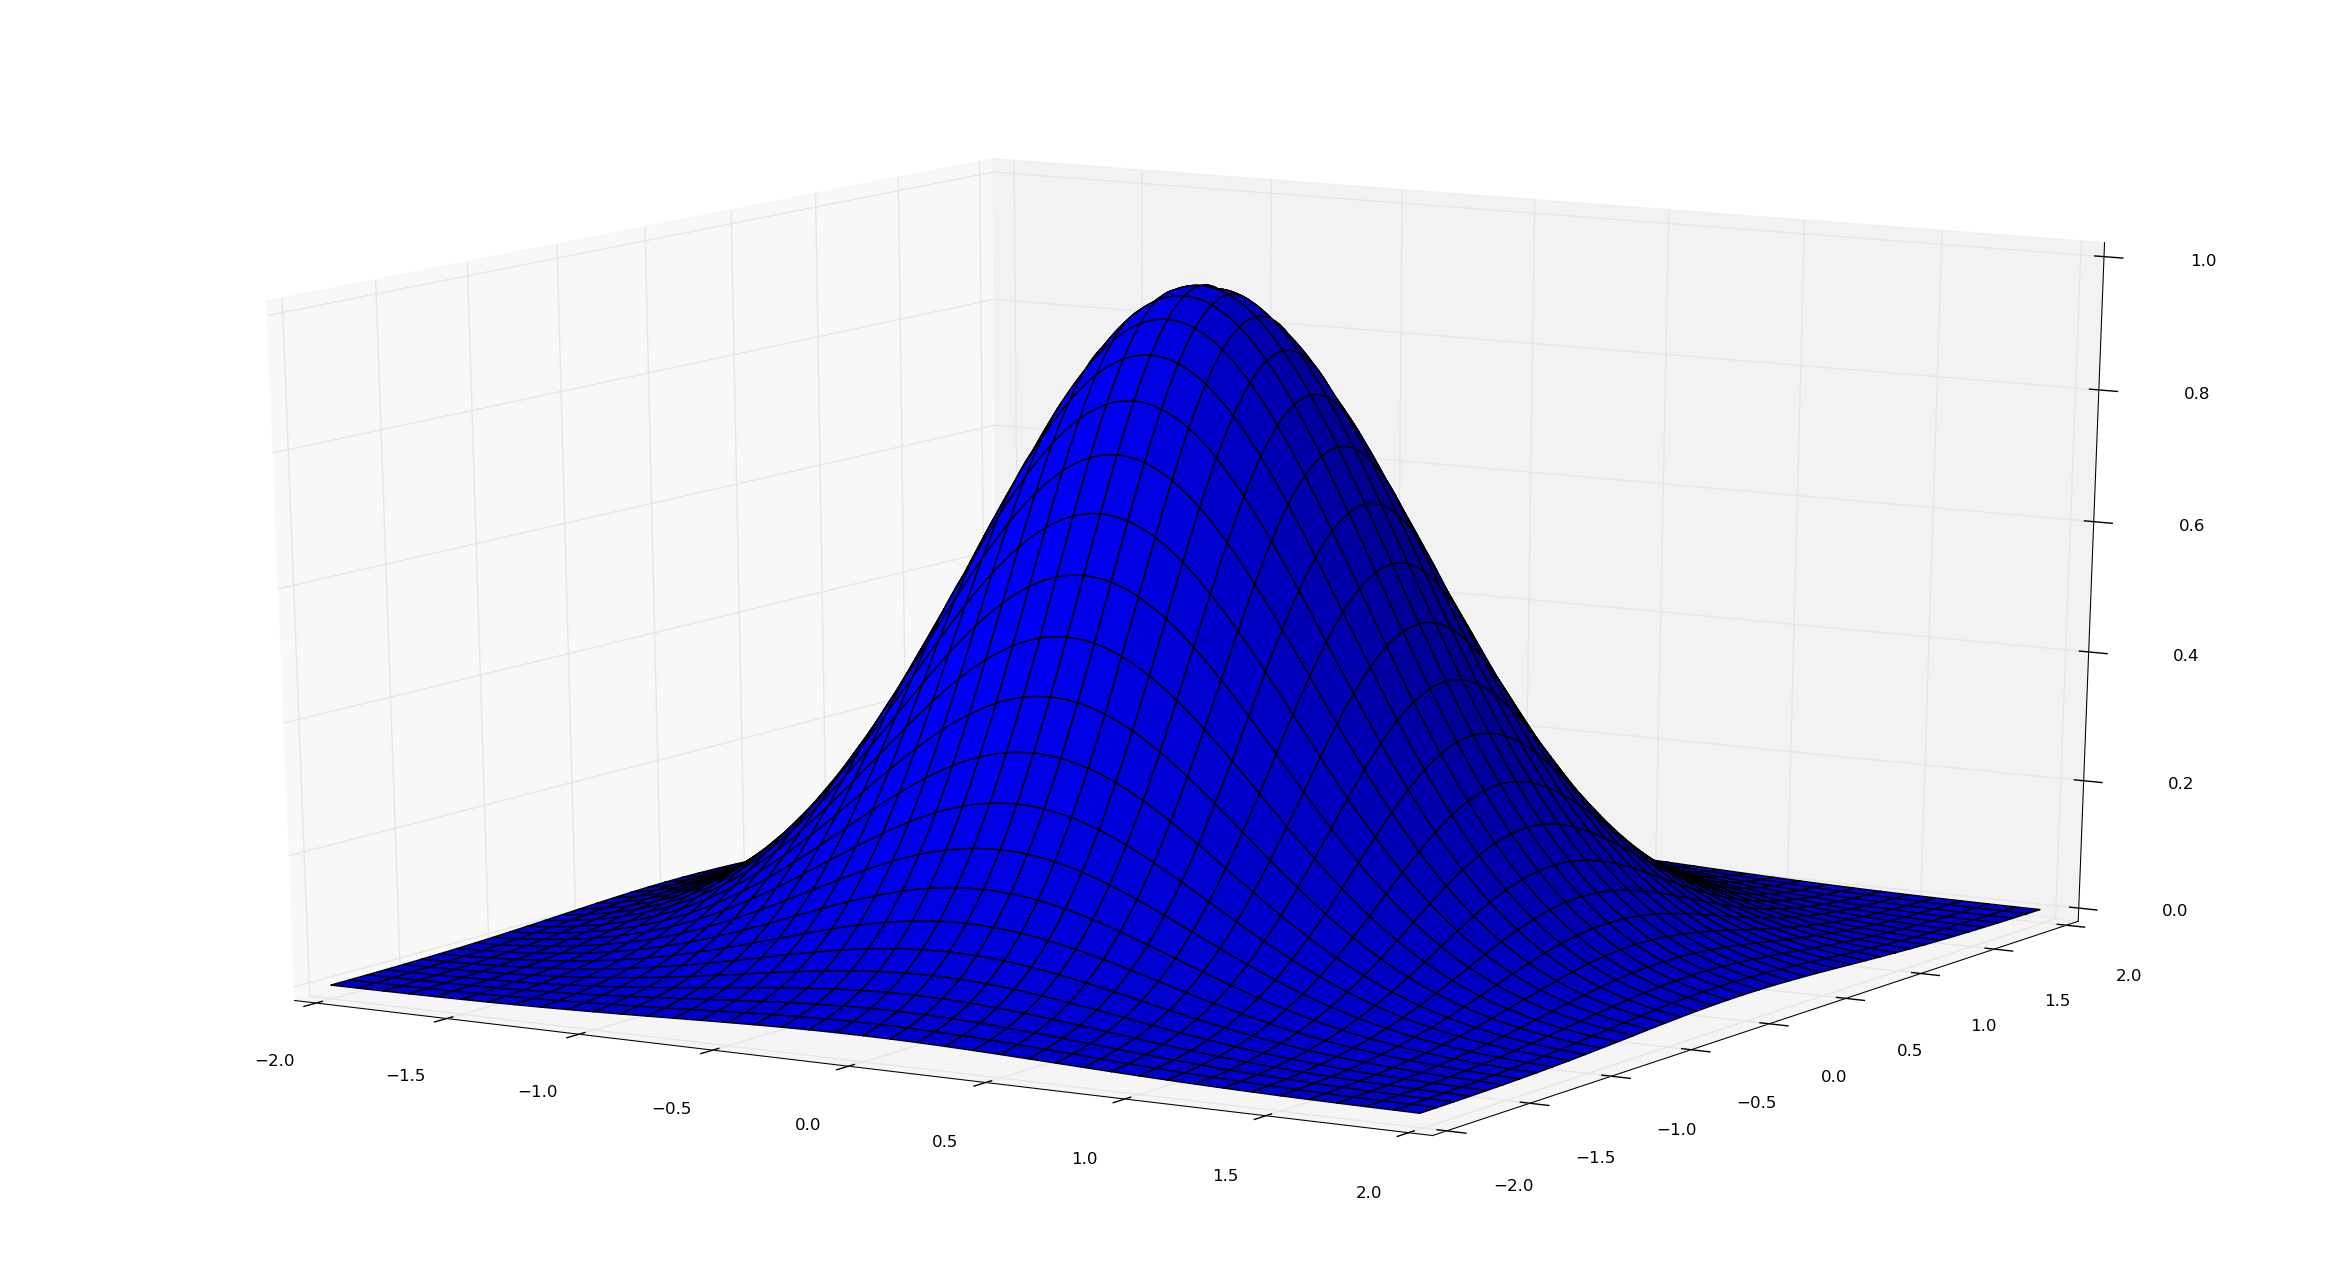
\includegraphics[width=\columnwidth]{figures/blob.png}%
\caption{RBF Kernel}%
\label{RBFKernel}%
\end{figure}
\end{frame}



\subsection{Learning words}

\begin{frame}{Learning words}
We have to build a prior lexicon that contains how characters interact to create words.
\begin{enumerate}
	\item Word database ICDAR 2003 word \cite{ICDARword}\footnote{\url{http://algoval.essex.ac.uk/icdar/Datasets.html}};
	\item compute for each pair of characters $(c_i,c_j)$ their frequency of occurrence $p(c_i,c_j)$ in the database (bi-gram model);
	\item will be used as an energy term to be minimized afterward.
\end{enumerate}
\end{frame}





\section{Character detection}

%\subsection{Sliding window and pruning}

\begin{frame}{Sliding window and pruning}
\begin{itemize}
	\item Scan the image with sliding windows;
	\item for each window $l_i$, compute $\phi_i$, feature of HOG with 12 orientations;
	\item run the 62 SVMs on $\phi_i$ and compute the goodness score:
	\begin{equation}
	GS(l_i) = \max_c p(c|\phi_i) \exp\left( - \frac{(a_i - \mu_{a_j})^2}{2\sigma_{a_j}^2} \right)
	\label{eq:}
	\end{equation}
	$a$ is the aspect ratio and $j$ is the class that reaches the maximum.
\end{itemize}
\end{frame}

\begin{frame}{Sliding window and pruning}
\begin{itemize}
	\item if $GS(l_i) > \texttt{threshold}$, keep the window \textbf{and} all the probabilities of each character.
	\item apply Non-Maximum Suppression algorithm (NMS) to merge overlapping windows:
	\begin{enumerate}
		\item find $l_i$ with maximum confidence.
		\item for all others $l_j$ compute:
		\begin{equation}
		\text{criterion} = \frac{l_i \cap l_j}{l_i \cup l_j}
		\label{eq:}
		\end{equation}
		\item if criterion > \texttt{threshold} \textbf{and} highest character is the same then merge the windows.
		\item the ending merged window has the highest confidence and is located at the barycenter of all the windows merged.
	\end{enumerate}
\end{itemize}
\end{frame}


\section{Recognizing words}


\begin{frame}{Graph construction and retrieval of the word}
\begin{alertblock}{PGM part}
Technical part of graphical model implemented for PGM course, here is a (very) short summary.
\end{alertblock}
\textbf{Input. } set of $n$ windows with possible characters.
\begin{enumerate}
	\item for each window, assign a node taking values in $\mathcal{K}_{\epsilon}$ ($\epsilon$ void label);
	\item build edges if the windows are 'close enough';
	\item assign unary energy to nodes, \textbf{and} pairwise energy for edges (overlapping terms + lexicon prior):
	\begin{equation}
	E(\mathbf{x}) = \sum_{i\in \mathcal{V}} E_i(x_i) + \sum_{(x_i,x_j)\in\mathcal{E}} E_{i,j}(x_i,x_j)
	\label{eq:}
	\end{equation}
	\item minimize the discrete energy on the graph (NP-hard) with TRW-S algorithm \cite{Kol}.
\end{enumerate}

\end{frame}




\section{Implementation and first results}

%\begin{frame}{Implementation}
%\begin{itemize}
	%\item Implementation in Python;
	%\item computing HOG => two parameters, size of the bins and number of orientations;
	%\item building $K$ with sci-kit learn => $2\times 62$ parameters to be optimized, done by 6-fold-cross-validation on an exponential search-grid;
	%\item threshold of GS (low) to keep first a window;
	%\item threshold for NMS;
	%\item parameters of graph construction.
%\end{itemize}
%\end{frame}


\begin{frame}{Implementation and first results}
\begin{figure}%

\includegraphics[width=\columnwidth]{figures/puffTest.png}%
\caption{Image for testing the algorithm}%
\label{}%
\end{figure}
\end{frame}

\begin{frame}{Implementation and first results}
\begin{figure}%

\includegraphics[width=\columnwidth]{figures/puff.png}%
\caption{Word retrieved: 'PE'}%
\label{}%
\end{figure}
\end{frame}


\begin{frame}{Implementation and first results}
\begin{figure}%
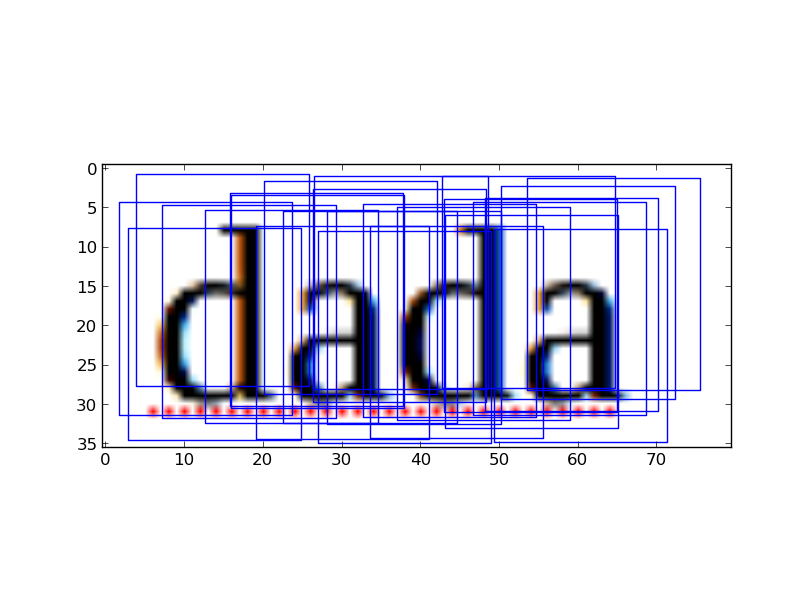
\includegraphics[width=9cm]{figures/dada2.png}%
\caption{All the sliding windows kept to build graphical model}%
\label{}%
\end{figure}
\end{frame}


\begin{frame}{Implementation and first results}
\begin{figure}%
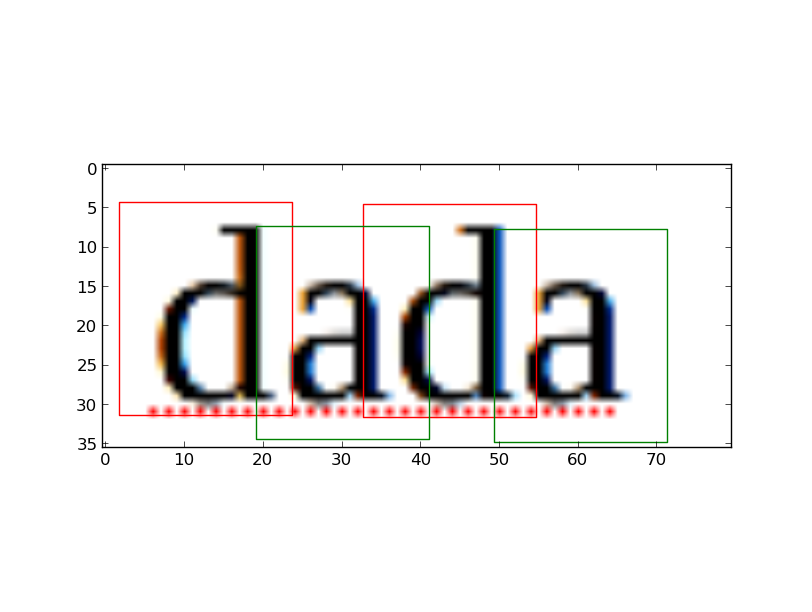
\includegraphics[width=9cm]{figures/dada1.png}%
\caption{Presence of the letters 'a' (green) and 'd' (red)}%
\label{}%
\end{figure}
\end{frame}



\begin{frame}{Implementation and first results}
\begin{figure}%
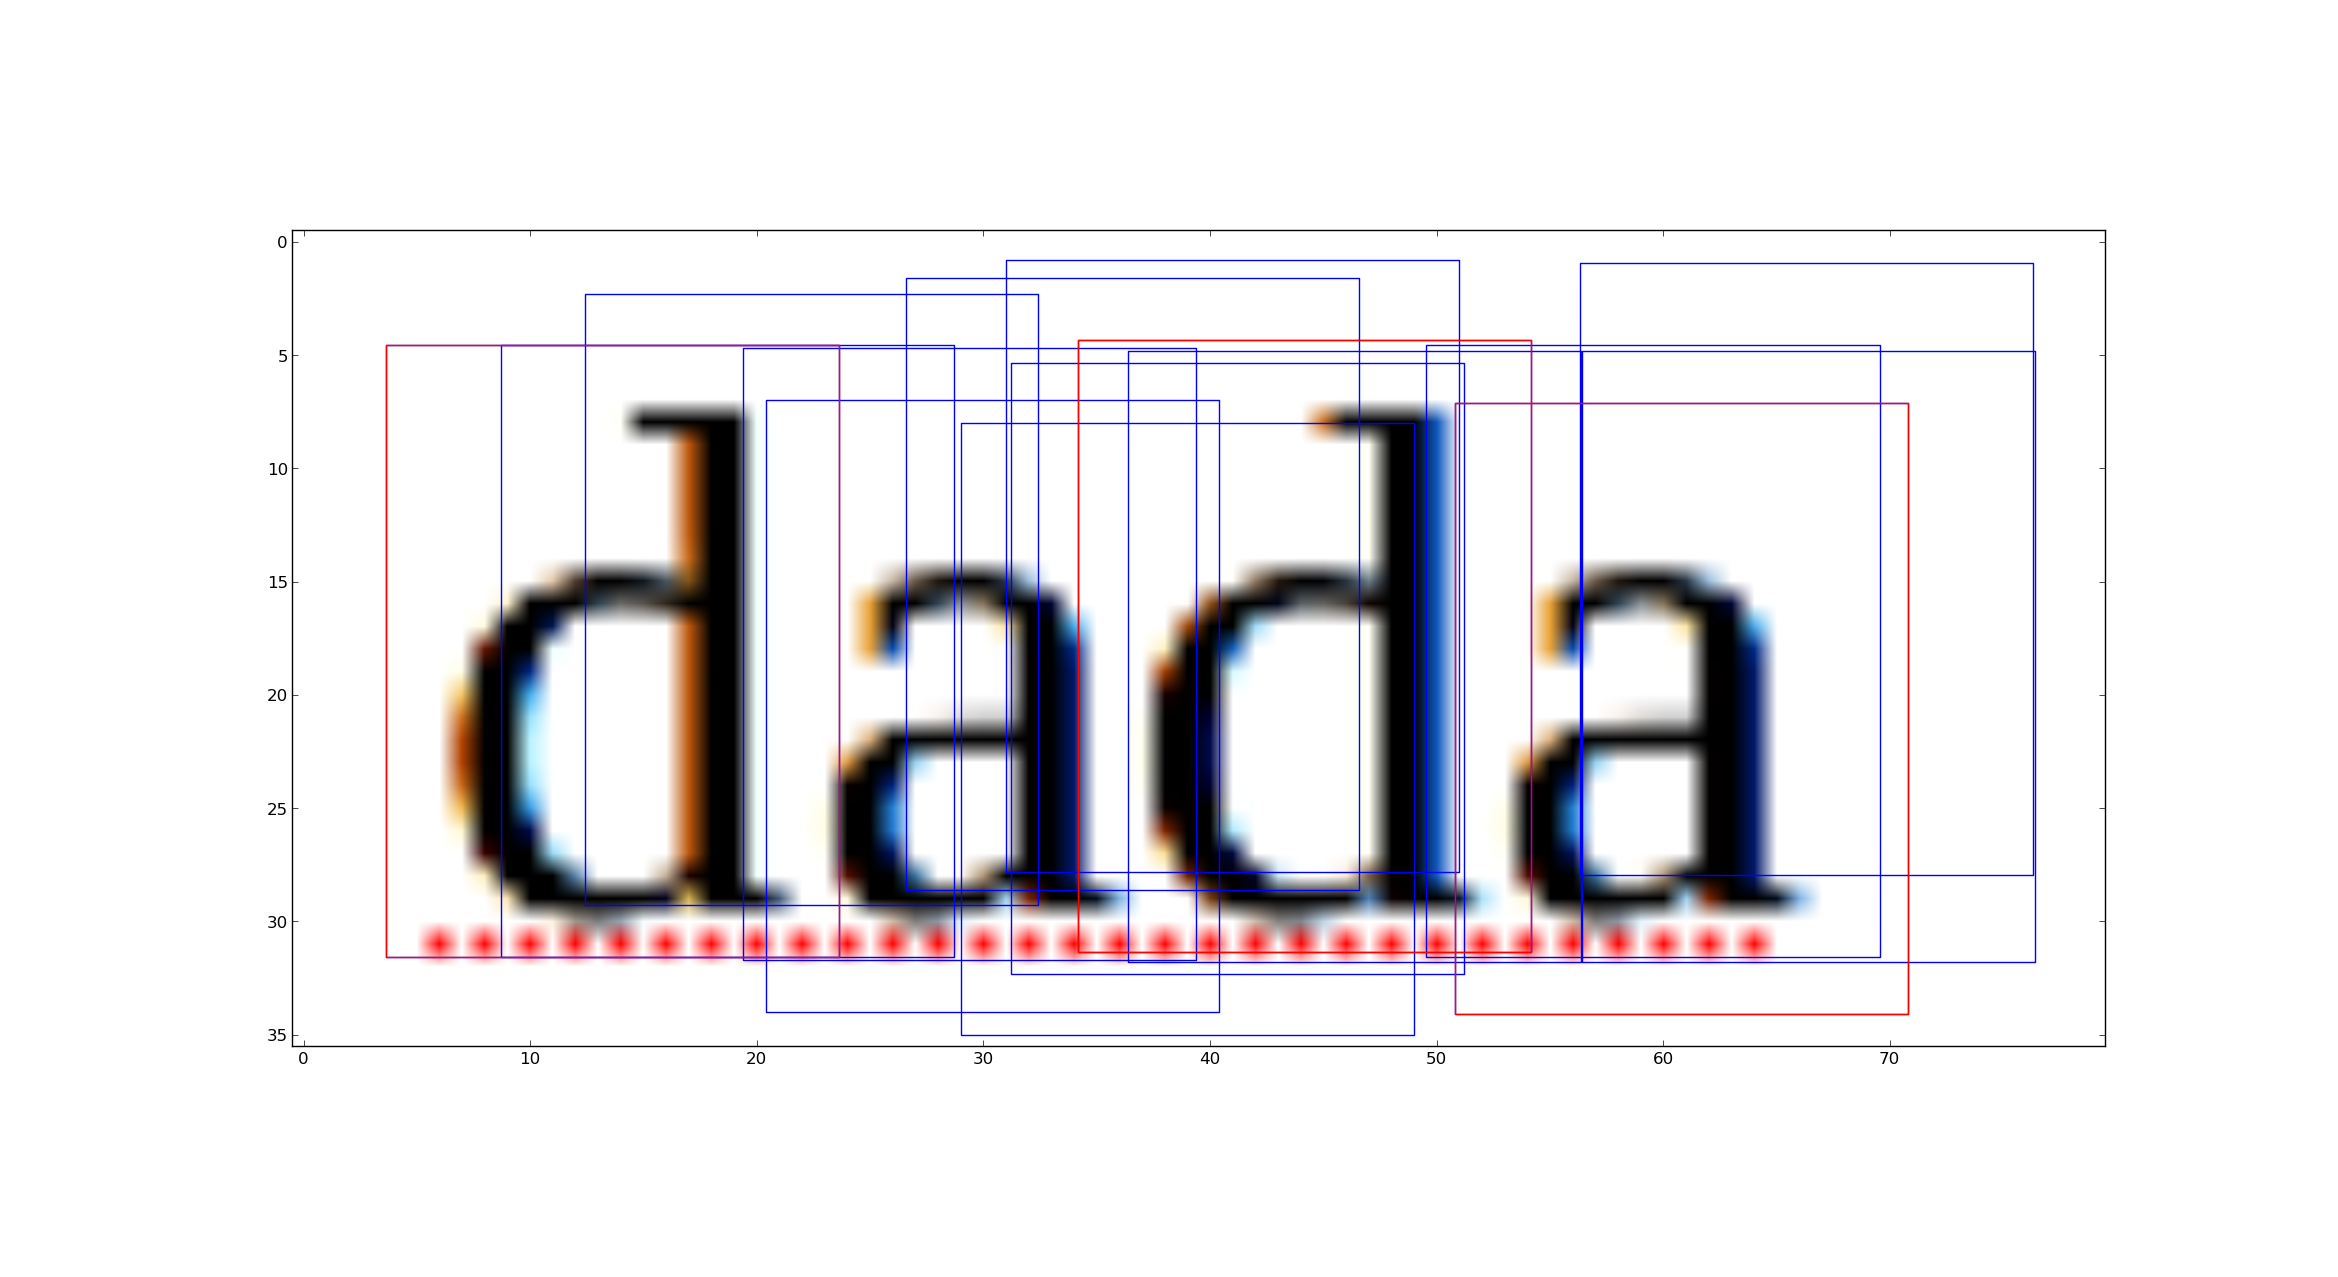
\includegraphics[width=9cm]{figures/dada3.png}%
\caption{Word retrieved 'dda' -> the second a has a too big overlap (penalized by pairwise energy, PGM part)}%
\label{}%
\end{figure}
\end{frame}


\begin{frame}{Improvements}
\begin{enumerate}
	\item \textbf{Difficult problem}: for each window, classify $K$ times. 
	
	\item SVM is not good enough (albeit a 14-hours cross-validation): error on the training set is still $16\%$.
		
	\item parameters of the algorithm: $2\times K$ for SVMs + 2 for HOG (bins, number of orientations) + threshold for GS + threshold in NMS + parameters of energy and of TRW-S => complex algorithm.
	
	\item (PGM part) The energy tends to explode letters instead of joining them into words (example 'dda').
\end{enumerate}
\end{frame}



\begin{frame}{Improvements}
\begin{figure}%
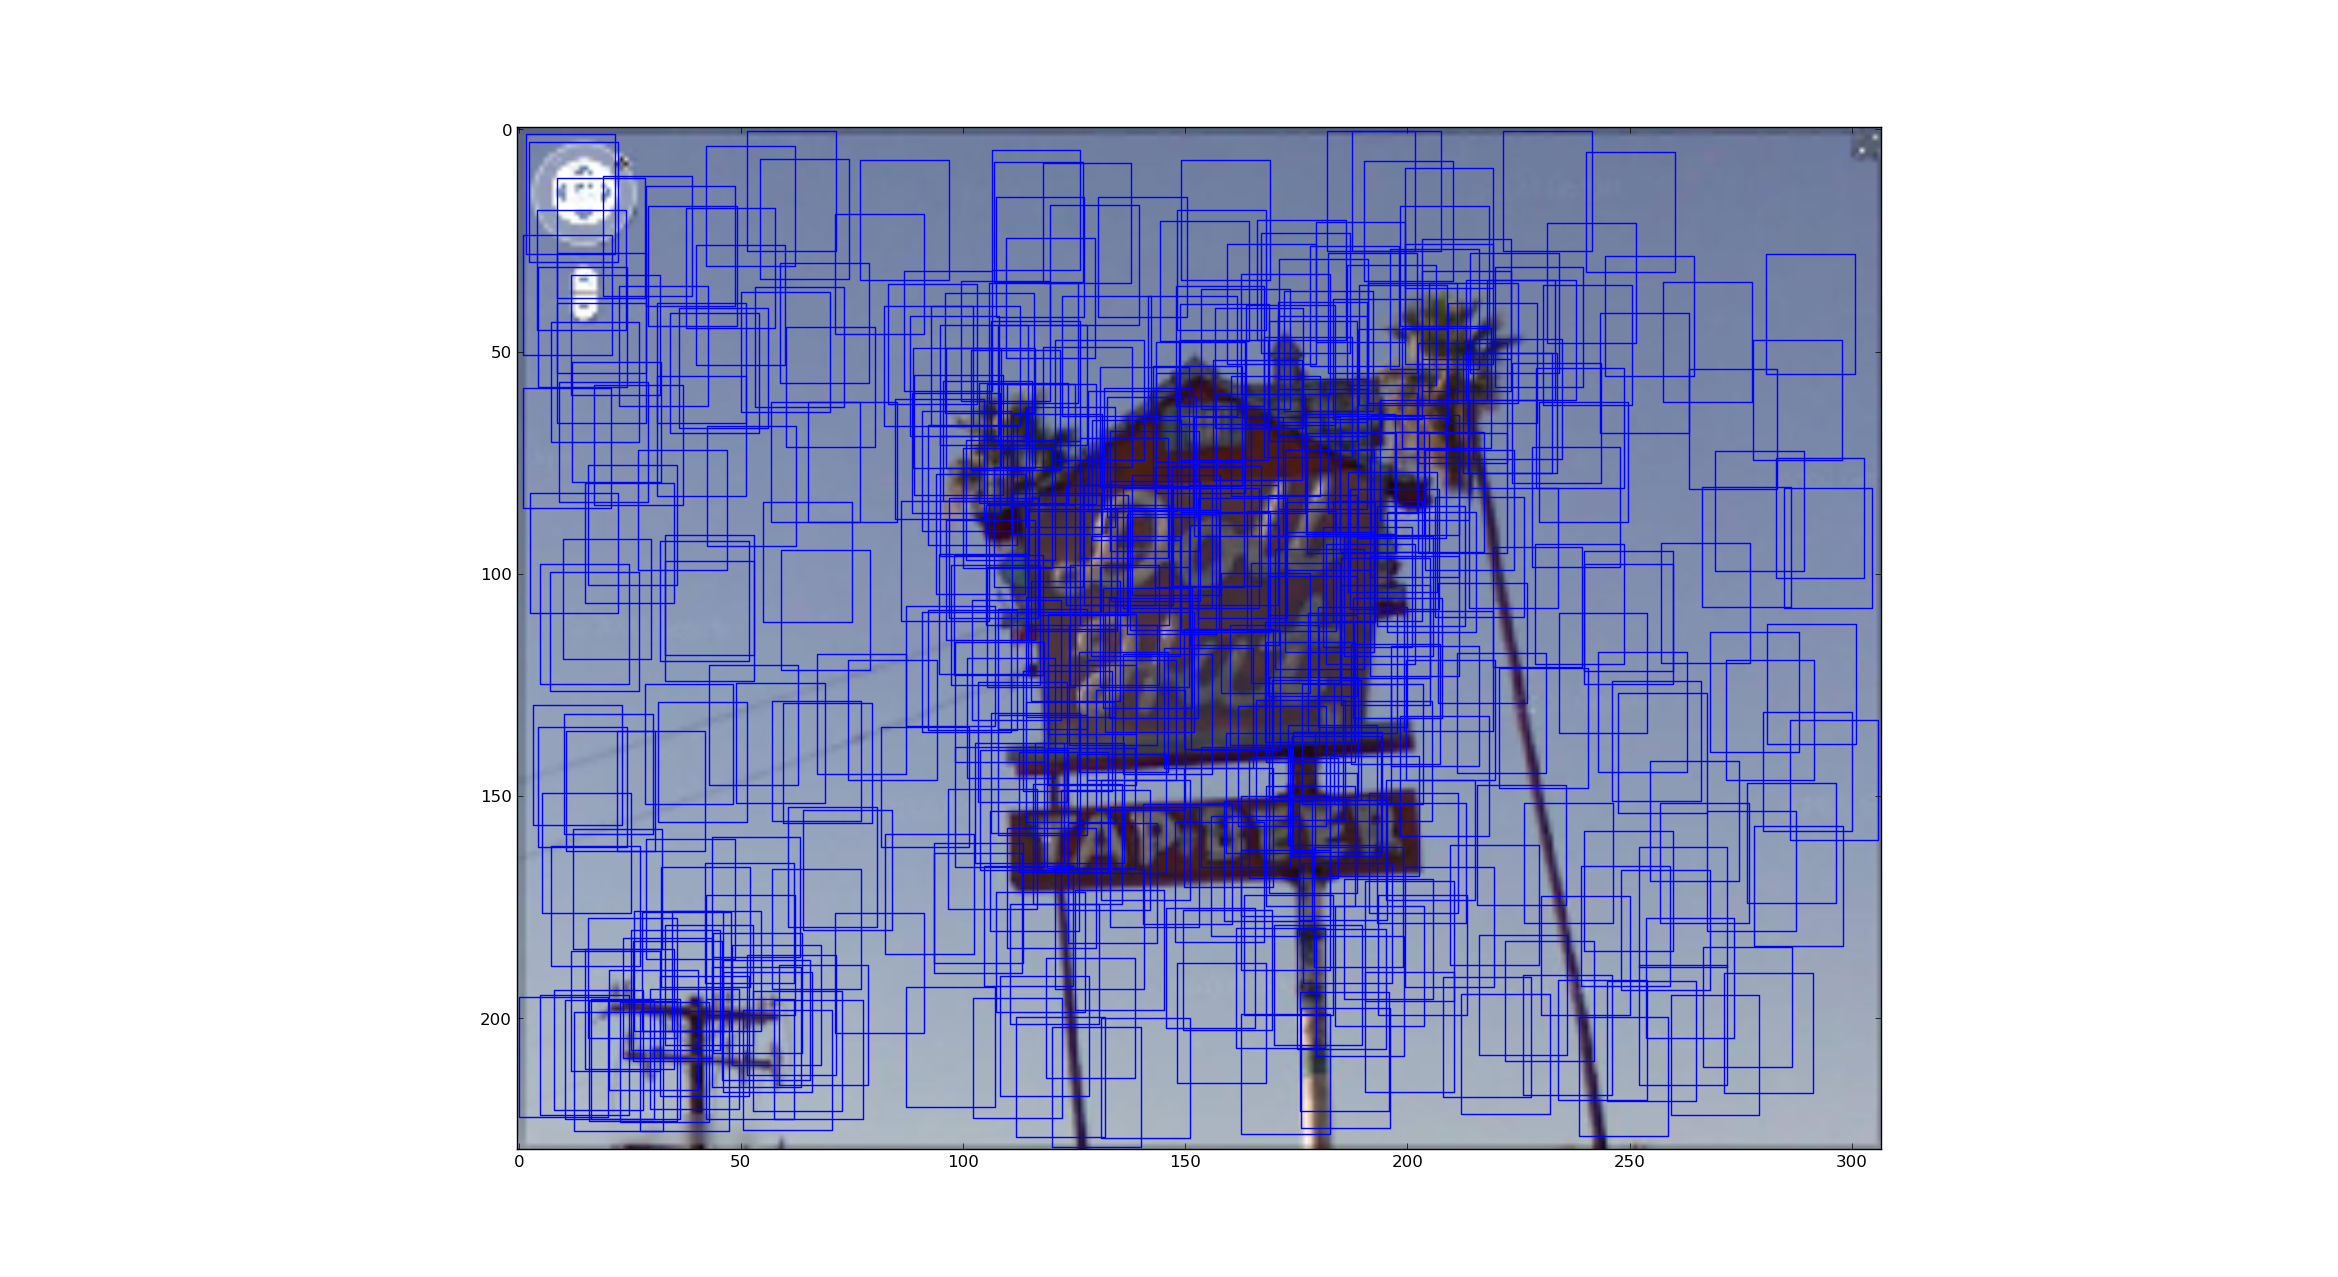
\includegraphics[width=\columnwidth]{figures/beer.png}%
\caption{Flexible GS threshold... too many windows}%
\label{}%
\end{figure}
\end{frame}





\begin{frame}{References}
\tiny
\bibliographystyle{unsrt}
\bibliography{biblio}
\end{frame}






\end{document}